\documentclass[12pt,a4paper]{article}
\usepackage[utf8]{inputenc}
\usepackage[russian]{babel}
\usepackage[OT1]{fontenc}
\usepackage{amsmath}
\usepackage{amsfonts}
\usepackage{amssymb}
\usepackage{graphicx}
\usepackage{mathtools}
\usepackage[left=2cm, right=2cm, top=2cm, bottom=2cm]{geometry}

 \newcommand{\tit}[1]{\begin{center}{\bf{\Large #1}}\end{center}}
 \newcommand{\aut}[1]{\centerline{{\bf #1}}}
 \newcommand{\cityorg}[1]{\centerline{\it #1}}
  \newcommand{\email}[1]{\centerline{{\small e-mail: #1}}\vspace{\baselineskip}}
\begin{document}

\sloppy

 \tit{Title goes here}
 \tit{Mantle cloak: Invisibility induced by a surface}
 \aut{Andrea Alu}
 \cityorg{Department of Electrical and Computer Engineering, 
 University of Texas at Austin,}
 \cityorg{1 University Station C0803, Austin,  Texas 78712, USA}
 \email{alu@mail.utexas.edu}

\begin{abstract}
Недавно для различных задач маскировки были применины экзотические взаимодействия волн
метаматериалов, но реализация метаматериалов в практической маскировке еще далека от
идеала. Текущие методы изготовления по своей природе основаны на объемных свойствах
метаматериалов, которые требуют хоть сколько-нибудь заметную электрическую толщину.
Я представляю здесь идею поверхности маскировки, показывая, что узорчатые 
метаматериалы могут давать те же эффекты маскировки в более простой и более тонкой 
геометрии. Токи, порожденные на неактивной поверхности, служат для резкого подавления 
видимости данного объекта. 
\end{abstract}

\setcounter{secnumdepth}{5}
\section{Введение}
Последние исследования в технологии метаматериалов показали, что невидимость,
прозрачность и маскировка могут быть получены разными способами, основанными на
сложном взаимодействии волн искуственных материалов и метаматериалов (смотори 
\cite{1,2}). Основанная на преобразованиях маскировка \cite{3}-\cite{6} является
самой популярной техникой, недавно была предпринята попытка расширить 
эксперементальную реализацию до видимых частот \cite{7}. Принциы работы такой 
маскировки заключен в электромагнитных свойствах объемных метаматериалов с заданным
спецефичным анизотропным и неоднородным профилем, который может направлять 
электромагнитные волны вокруг заданной области пространства, изолируя и делая
невидимым любой объект, помещенный в такую область. Другим жизнеспособным методом
маскировки является плазмонная \cite{8,9}, основанная на аннулировании рассеяния 
особенностей низко-проницаемых метаматериалов, которые могут быть поляризованы 
необычными способами, а так же аномально локализованные резонансные мезанизмы 
\cite{10}, основанные на квазистатических резонансных свойствах метаматериалов, 
которые могут эффективно маскировать заданную область. Все эти техники, так же как
и многие другие, включающие плащ из метаметериалов, основаны на специфичных объемных 
свойствах слоев метаматериалов.
В общем, эти искуственные метаматриалы основаны на коллективном электромагнитном
ответе составляющих их включений, которые взаимодействуют с падающими 
электромагнитными волнами как объем, получая эффект, кардинально отличающийся от
эффекта, получаемого от индивидуальных материалов, из которых они составлены.
С одной стороны, это может давать большую степень свободы для получения анольмальных
эффектов, таких как маскировка, с другой стороны плащи из метаматериалов изначально 
требуют определенной тонкости, из-за конечного размера составяющих включений. 
В случае с основанными на преобразованииплащами плащами, в частности, вовлеченный 
неоднородный профиль требует плащ, который имеет толщину, сравнимую по размеру с 
маскируемой областью. Более того, обычно требуется некоторое пространтсво между
плащом из метаматериалов и маскируемым объектом, чтобы гарантировать, что 
зернистость материала не порождает нежелаемых сцепок с объектом, которые могут 
повлиять на его электромагннитный свойства в целом \cite{11}. Более тонкий плащ
это не только непрактично и нежелательно, но также означает уменьшение пропускной
способности и увеличение чувствительности \cite{12}. Даже техника плазмонной 
маскировки, которая требует относительно тонкого плаща, по сравнению с основанными
на преобразовании метаматериалами, может требовать на практике конечной толщины
для 	надлежащей работы \cite{11,13}.

В другой области, понятие узорной тонкой металлической поверхности хорошо известно
в различных инжинерных приложениях, с соответствующими книгами и обзорами по этой
теме (смотри \cite{14}). При условии, что периодичесеский рисунок на металлической
поверхности намного меньше, чем длина волны, ее электромагнтиное поведение может
быть эффективно описано через усредненный импеданс поверхности $Z_s = R_s - iX_s$,
который связывает среднее тангенциальное электрическое поле на поверхности c 
средней плотностью индуцированного электрического тока как $\textbf{E}_{tan}=
Z_s\textbf{J}$. Импеданс $Z_s$ обычно предполагает широкий диапазон значений, как
функция пространства и частоты, из которой происходит название <<Частотно-
изберательная поверхность>>(frequency selective surface (FSS)). 
В лучшем случае, легко показать, что $Z_s$ чисто мнимое, $R_s$
относится только к поглащению. В более общем случае, однако, значение $Z_s$ может зависеть от ориентации
тангенциального электрического поля, предполагающую анизотропную и тензорную структуру 
$\underline{\textbf{Z}}_s$. Скалярная запись может быть приемлимой для особых поляризаций падающей волны.

Далее, я покажу что единичной узурчатой FSS может быть достаточно, чтобы произвести эффект маскировки,
аналогичный эффекту с плащом из метаматериалов, даже в идеальном пределе с поверхностью нулевой толщины.
Это может породить тонкие плащи в полученных технологих с длинными историями применений,
обещает более легкую реализацию, возможное прилегание к форме объекта, низкий профиль и относительно
больший диапазон работы. Схожие идеи могут быть расширены на металлические поверхнгости тетрагерцевых
и оптических частот, открытие перспектив для реализации тонких плащей с повышенной производительностью.
Мантевая маскировка (\textit{mantle cloak}), которая предложена здесь может приблизить нас к практической
реализации маскировки, так как она не будет опираться на свойства, определяющих материал, а только на
поперечное сопротивление узорной металлической поверхности. Следует упомянуть, что мягкий и трудный
FSS уже применялисть в прошлом в устройствах снижения рассеяния \cite{15}, но использовали идеи,
решительным образом отличающиеся от примененных здесь. Здесь же, интерес заключается в реализации
механизма маскировки, который не зависит от угла падения и, возможно, от поляризации волны, что будет
описано далее.

\begin{figure}[t]
  \centering
  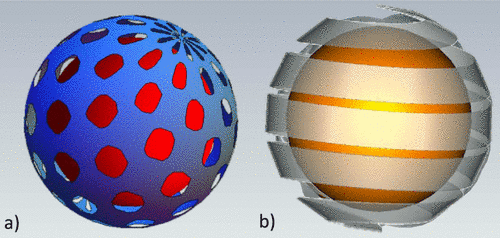
\includegraphics[height=0.15\paperheight]{1.png}
  \caption{Примеры узорных геометрических форм, которые могут реализовать мантевую маскировку.}
  \label{fig:1}
\end{figure}

\section{Теоретические формулировки}
Рассмаотрим примеры геометрических форм в Рис.\ref{fig:1}, т.е. диалектрические сферы радиусом $a$,
покрытые узорчатой металлической сферической поверхностью незначительной толщины радиуса $a_c > a$.
Они представляют собой типичные шаблоны, которые могут быть реализованы на металлической поверхности
для получения квазиоднородной поверхности с реактивным сопротивлением заданного значения. Доказано, что
шаблоны являются субволновыми, они могут создать квазиоднородную поверхнгость с реактивным сопротивлением
заданного значения.

Один предельный случай возникает, когда проводящая поверхность не имеет отверстий, которые мы могли
обеспечить эффективное нулевое тангенциальное електрическое поле, дающее $X_s = 0$. В другом крайнем
случае, когда метал отсутствует вовсе, реактивное сопротивление поверхности $X_s \to \infty$.
Как показано в \cite{14} и находящихся в ней ссылках, надлежащий выбор шаблонов на мателлической
поверхности позволяет достигнуть желаемого положительного или отрицательного значения $X_s$ на 
интересуемой частоте. После гомогенизации задача рассеяния заданного произвольного возбуждения может
быть решена аналитически, введением желаемого скачка касательного магнитного поля на поверхности плаща
в $r=a_c$, пропорциольного среднему току, индуцированному на поверхности. Это означает, что граничное
условие 
\begin{equation}
\left.\textbf{H}_{tan}\right|_{r=a_c^+} - \left.\textbf{H}_{tan}\right|_{r=a_c^-} = 
\hat{r} \times \left.\textbf{E}_{tan}\right|_{r=a_c} / Z_s
\end{equation} 	
выполняется в изотропном случае. Решение Ми этой задачи означает, что н-тая 
поперечно-магнитная(Transverse-Magnetic) сферическая гармоника может быть подавлена при условии,
что следущий определитель аннулируется(?):
\begin{equation}\label{eq2}
\begin{vmatrix}
j_n(ka) & j_n(k_0a) & y_n(k_0a) & 0\\
[kaj_n(ka)]'/\varepsilon & [k_0aj_n(k_0a)]' & [k_0ay_n(k_0a)]' & 0\\
0 & j_n(k_0a_c)+\frac{[k_0a_cj_n(k_0a_c)]'}{iw\varepsilon_0a_cZ_s} &
y_n(k_0a_c) + \frac{[k_0a_cy_n(k_0a_c)]'}{iw\varepsilon_0a_cZ_s} & j_n(k_0a_c)\\
0 & [k_0a_cj_n(k_0a_c)]' & [k_0a_cy_n(k_0a_c)]' & [k_0a_cj_n(k_0a_c)]'
\end{vmatrix},
\end{equation}
где $j_n(\cdot)$ и $y_n(\cdot)$ сферические функции Бесселя, $k$ и $k_0$ волновые числа в объекте и
своободном пространтсве соотвественно, $\varepsilon$ --- диалектрическая проницаемость объекта,
$\varepsilon_0$ --- диалектрическая проницаемость свободного пространства.
Для поперечно-электрической(transverse-electric(TE)) гармоники можно легко 
получить сопряженное к уравнению $\ref{eq2}$. При условии, что детерминант в уравнении 
\ref{eq2} может быть приближен к нулю для старших порядков рассеяния, видимость заданного
объекта будет резко уменьшена, в независимости от поляризации, вида возбуждений и позиции
наблюдателя, при этом достигается хоть и не идеальный, из-за остаточных членов рассеяния,
эффект маскировки. Может быть так же предусмотрено расширение до анизотропных поверхностей
и тензора $\underline{\textbf{Z}}_s$, производящее в целом поперечное соединение двух 
поляризаций. Следует заметить, однако, что изотропная формулировка в \ref{eq2} применима
даже для анизотропных поверхностей с спецефическими поляризациями входящей волны.

Полезно проанализировать формулу \ref{eq2} в квазистатическом пределе(электрически маленькие 
объекты), для которых $(k_0a_c) \ll 1$. В этом случай основной вклад в рассеяние дает
$n=1$ доминантная гармоника и приближенные условия для маскировки для маскировки в 
случае двух поляризаций можно записать в явном виде как
\begin{equation*}
TM:X_s = 
\frac{2[2+\varepsilon-\gamma^3(\varepsilon-1)]}{3\gamma^3\omega a\varepsilon_0(\varepsilon-1)
}
\end{equation*}
\begin{equation}\label{eq3}
TE:X_s = \frac{\omega a\mu_0[2+\mu+2\gamma^3(\mu-1)]}{6\gamma^3(\mu-1)}
\end{equation}
где $\mu$ означает проницаемость, а $\gamma=a/a_c$.

Уравнение $\ref{eq3}$ показывает, что в квазистатическом пределе вклад TE и TM гармоник в 
рассеяние разделяется, как и ожидалось, и это гарантирует, что доминирующие мультиполярные
члены, как эдектрические так и магнитные, оба могут быть подавлены, при правильном выборе
реактивного сопротивления FSS.Несмотря на то, что нулевое рассеяние образуется при помощи 
тонкой поверхности, конформной объекту, оно может быть достигнуто в этом пределе без потерь 
реактивной поверхности, и наличие реалистичных потерь в металле не повлияет на эффект 
маскировки. Когда размер объекта увеличивается, динамические формулы как в \ref{eq2} могут
быть использованы для правильного построения плаща. Эта формулировка может быть расширена на
случай проводящих объектов и различных несимметричных геометрий и анизотропий без изменения
результата.

\begin{figure}[t]
  \centering
  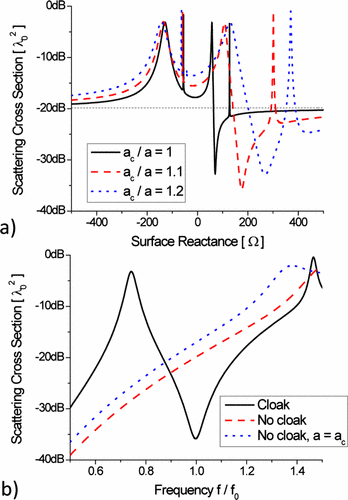
\includegraphics[height=0.3\paperheight, width=0.4\paperwidth]{2.png}
  \caption{Изменение в общем рассеяния поперечного сечения непроводящей сферы с $\varepsilon
  =10$ и $2a=\lambda_0/5$ с: (a) реактивным сопротивлением поверхности mantle cloak; (b)
  нормализованной частотой для операций на плаще с $a_c=1.1a$ и $X_s=175\Omega$}
  \label{fig:2}
\end{figure}

\end{document}